% !TeX spellcheck = en_US
%%
%% sample document for AAMAS'18 conference
%%
%% modified from sample-sigconf.tex
%%
%% see ACM instructions acmguide.pdf
%%
%% AAMAS-specific questions? n.yorke-smith@tudelft.nl
%%

\documentclass[sigconf]{aamas}  % do not change this line!

%% your usepackages here, for example:
\usepackage{booktabs}
\usepackage{graphicx}
\usepackage[rflt]{floatflt}
\usepackage{subcaption} 
\usepackage{frame, caption}
\usepackage{amsmath}
\usepackage{mathrsfs}
\usepackage{array}

\newcommand{\argmax}{\operatornamewithlimits{arg\,max}}

%% do not change the following lines
\setcopyright{ifaamas}  % do not change this line!
\acmDOI{doi}  % do not change this line!
\acmISBN{}  % do not change this line!
\acmConference[AAMAS'18]{Proc.\@ of the 17th International Conference on Autonomous Agents and Multiagent Systems (AAMAS 2018), M.~Dastani, G.~Sukthankar, E.~Andre, S.~Koenig (eds.)}{July 2018}{Stockholm, Sweden}  % do not change this line!
\acmYear{2018}  % do not change this line!
\copyrightyear{2018}  % do not change this line!
\acmPrice{}  % do not change this line!

%% the rest of your preamble here


%%%%%%%%%%%%%%%%%%%%%%%%%%%%%%%%%%%%%%%%%%%%%%%%%%%%%%%%%%%%%%%%%%%%%%%%%%%%%%%%%%%%%%%%%%%%%%%%%%%%%%%%%

%%%%%%%%%%%%%%%%%%%%%%%%%%%%%%%%%%%%%%%%%%%%%%%%%%%%%%%%%%%%%%%%%%%%%%%%%%%%%%%%%%%%%%%%%%%%%%%%%%%%%%%%%

\begin{document}
	
	\title{I've got the power's value! A computational model to evaluate the interlocutor's behaviors in collaborative negotiation}  % put your title here!

	\subtitle{Socially Interactive Agents Track}

	
	% AAMAS: submissions are anonymous for most tracks
	\author{Paper \#32}  % put your paper number here!
	

	%
	%\author{Ben Trovato}
	%\authornote{Dr.~Trovato insisted his name be first.}
	%\orcid{1234-5678-9012}
	%\affiliation{%
	%  \institution{Institute for Clarity in Documentation}
	%  \streetaddress{P.O. Box 1212}
	%  \city{Dublin} 
	%  \state{Ohio} 
	%  \postcode{43017-6221}
	%}
	%\email{trovato@corporation.com}
	%
	%\author{G.K.M. Tobin}
	%\authornote{The secretary disavows any knowledge of this author's actions.}
	%\affiliation{%
	%  \institution{Institute for Clarity in Documentation}
	%  \streetaddress{P.O. Box 1212}
	%  \city{Dublin} 
	%  \state{Ohio} 
	%  \postcode{43017-6221}
	%}
	%\email{webmaster@marysville-ohio.com}
	%
	%\author{Lars Th{\o}rv{\"a}ld}
	%\authornote{This author is the
	%  one who did all the really hard work.}
	%\affiliation{%
	%  \institution{The Th{\o}rv{\"a}ld Group}
	%  \streetaddress{1 Th{\o}rv{\"a}ld Circle}
	%  \city{Hekla} 
	%  \country{Iceland}}
	%\email{larst@affiliation.org}
	%
	%\author{Valerie B\'eranger}
	%\affiliation{%
	%  \institution{Inria Paris-Rocquencourt}
	%  \city{Rocquencourt}
	%  \country{France}
	%}
	%\author{Aparna Patel} 
	%\affiliation{%
	% \institution{Rajiv Gandhi University}
	% \streetaddress{Rono-Hills}
	% \city{Doimukh} 
	% \state{Arunachal Pradesh}
	% \country{India}}
	%\author{Huifen Chan}
	%\affiliation{%
	%  \institution{Tsinghua University}
	%  \streetaddress{30 Shuangqing Rd}
	%  \city{Haidian Qu} 
	%  \state{Beijing Shi}
	%  \country{China}
	%}
	%
	%\author{Charles Palmer}
	%\affiliation{%
	%  \institution{Palmer Research Laboratories}
	%  \streetaddress{8600 Datapoint Drive}
	%  \city{San Antonio}
	%  \state{Texas} 
	%  \postcode{78229}}
	%\email{cpalmer@prl.com}
	%
	%\author{John Smith}
	%\affiliation{\institution{The Th{\o}rv{\"a}ld Group}}
	%\email{jsmith@affiliation.org}
	%
	%\author{Julius P.~Kumquat}
	%\affiliation{\institution{The Kumquat Consortium}}
	%\email{jpkumquat@consortium.net}
	%
	%% The example's default list of authors is too long for headers
	%\renewcommand{\shortauthors}{B. Trovato et al.}
	
	
	\begin{abstract}  % put your abstract here!
		
	
		
	\end{abstract}
	

	\keywords{Dominance; Reasoning about other; Theory of mind}  % put your semicolon-separated keywords here!
	
	\maketitle

	
	\section{Introduction}
	
	Negotiation is a common task in daily life. People negotiate not only in professional situations (\emph{e.g.} for a salary increase or a promotion) but also in more simple situations such as choosing the holiday's destination. In the last decade, a variety of conversational agents which negotiate with people  have been created \cite{pynadath2013you,gratch2016misrepresentation,klatt2011negotiations}.
	
	However, negotiation is a multifaceted process which also involves social interaction, affects as well as personal preferences and opinions  \cite{bro2010affective}. Several research considered the of role social behavior in the negotiation process, such as emotions and trust	\cite{de2011effect}. Research in social psychology demonstrated that the relation of dominance affects the way that the negotiation process is perceived \cite{van2006power}. Negotiators build different negotiation strategies depending on their relative dominance which directly influences the outcomes of the negotiation. More precisely, Tidens \cite{tiedens2003power} showed that dominance complementarity (\emph{i.e.} one negotiator exhibits dominant behaviors while the other one responds with submissive ones) leads the negotiators to reach mutually beneficial outcomes and increases their reciprocal likings.
	
	Dominance, as an interpersonal relation, is a dyadic variable in which control attempts by one individual are accepted by the partner. This means that one individual expresses behaviors of high power while the interactional partner adopts a low power behavior \cite{burgoon1998nature}. 
	
	In this poster, we present an agent that simulates such a relation of dominance when negotiating with a human interlocutor. The agent is able to express and understand behaviors related to power. This work is based on the computational model proposed by \cite{ouali2017computational} in which an agent expresses its behavior of power through its strategy of negotiation. It is based on three principles of negotiation based on power inspired from social psychology \cite{de1995impact,van2006power,magee2007power}. We show how this model can be adapted to reason about the user's power, following a Theory of Mind approach. We simulate the mental activity of the interlocutor, we show that the agent can make good predictions in the context of agent-agent interaction. We propose to use this model in the context of human-agent negotiation.
	
	\begin{figure*}
		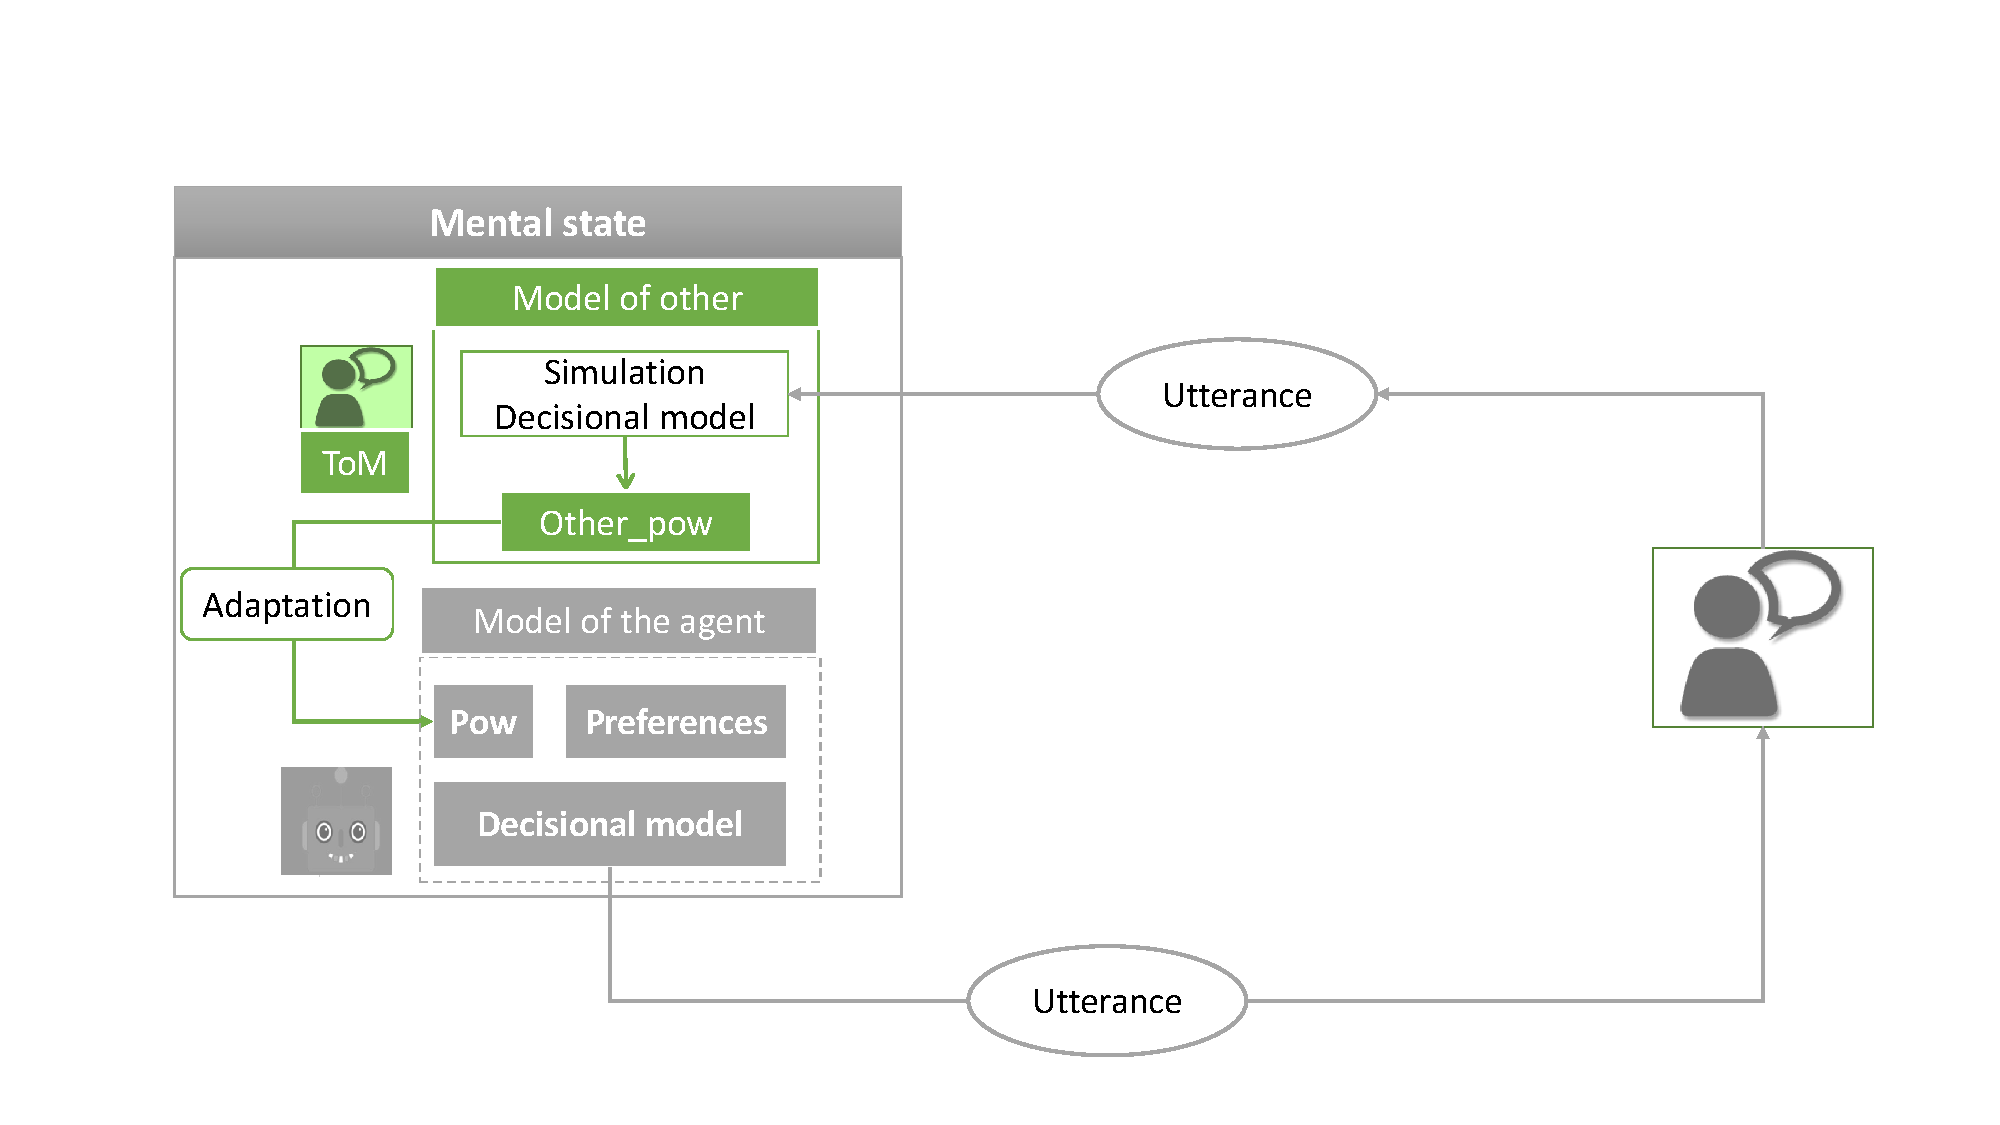
\includegraphics[width=0.65\linewidth, height= 0.25\textheight]{figs/model_tom.pdf}
		\caption{Model of collaborative negotiation with a model of other} 
		\label{fig:schema-general}
	\end{figure*} 


	\section{Negotiator agent with ToM}
		Present mental state of the agent (domain, communication) 
		
		Decision during the negotiation is built to take into account the preferences of the agent as well as his power. 
		Conclusion 1: in order to guess the user power, based on its behaviors (produced utterances) the agent has to make hypotheses about its mental state (preferences, power). Since, our aim is to guess the power, we propose a model in which the agent has a partial representation of preferences. 
		
		We propose an adaptation of the agent decision model to handle partial knowledge of preferences. 
		
	\section{Conclusion}

	
	%%%%%%%%%%%%%%%%%%%%%%%%%%%%%%%%%%%%%%%%%%%%%%%%%%%%%%%%%%%%%%%%%%%%%%%%%%%%%%%%%%%%%%%%%%%%%%%%%%%%%%%%%
	%% bibliography: see CFP for number of permitted pages
	
	\bibliographystyle{ACM-Reference-Format}  % do not change this line!
	\bibliography{bibliography}  % put name of your .bib file here
	
\end{document}